%% The PHY design logic — COLUMN variant, SUMMARY level (a demo paper needs the
%% shape of the design, not the thread launch order). One symmetric loop:
%% down the transmit side, across the air, up the receive side, and the ACK
%% closes it at the top. Colours say which layer owns a stage.
\documentclass[tikz,border=4pt]{standalone}
\usepackage{xcolor}
%% Shared look for the UnionLabs system figures. \input by each fig-*.tex so a
%% colour or a corner radius is changed in one place.
\usetikzlibrary{positioning,arrows.meta,fit,backgrounds,calc}

\definecolor{uCode}{HTML}{1F6F5C}     % the experimenter's own code
\definecolor{uApi}{HTML}{6B4BA8}      % the contract / ARQ layer
\definecolor{uPhy}{HTML}{2E5E9E}      % transports / DSP
\definecolor{uRadio}{HTML}{B4700F}    % hardware
\definecolor{uShare}{HTML}{8A2E4D}    % the shared workspace

\tikzset{
  blk/.style={draw, rounded corners=2pt, align=center, font=\small,
              minimum height=8mm, inner sep=3pt, fill=black!2},
  code/.style={blk, draw=uCode, thick, fill=uCode!6},
  api/.style={blk, draw=uApi, very thick, fill=uApi!7},
  phy/.style={blk, draw=uPhy, thick, fill=uPhy!6},
  radio/.style={blk, draw=uRadio, thick, fill=uRadio!8},
  share/.style={blk, draw=uShare, thick, fill=uShare!6},
  stage/.style={blk, minimum height=9.5mm, font=\scriptsize, text width=16mm,
                inner sep=2pt},
  flow/.style={-{Latex[length=2mm]}, thick},
  back/.style={-{Latex[length=2mm]}, thick, densely dashed},
  % labels that sit ON an arrow: opaque, so the line never strikes the text
  onarrow/.style={font=\scriptsize\itshape, fill=white, inner sep=1.5pt},
  lbl/.style={font=\scriptsize\itshape, inner sep=1pt},
  note/.style={font=\scriptsize, align=left, inner sep=1pt},
  legend/.style={draw, minimum width=3mm, minimum height=3mm, inner sep=0pt},
}
\newcommand{\mono}[1]{{\ttfamily\footnotesize #1}}
\newcommand{\monos}[1]{{\ttfamily\scriptsize #1}}

\begin{document}
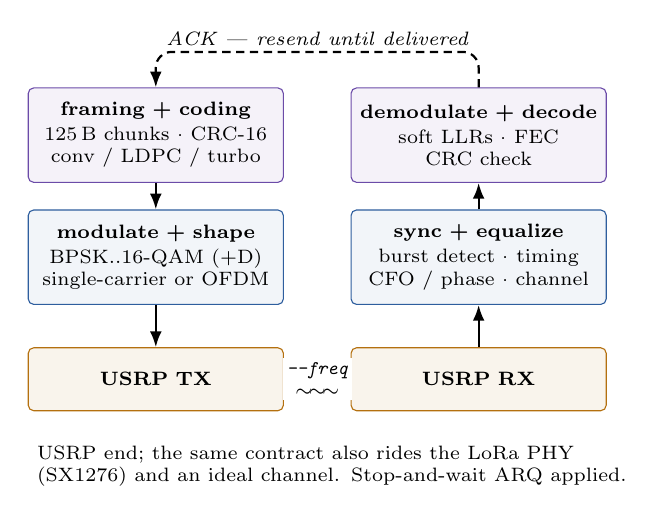
\begin{tikzpicture}[x=1mm, y=1mm,
  stage/.append style={text width=31mm, minimum height=12mm}]

\def\R{41}    % x of the receive column
\def\H{15.5}  % row pitch

%% ── transmit, top to bottom ──────────────────────────────────────────────
\node[stage, fill=uApi!7, draw=uApi] (arq) at (0,0)
  {\textbf{framing + coding}\\[1pt]
   {\scriptsize 125\,B chunks · CRC-16\\ conv / LDPC / turbo}};
\node[stage, fill=uPhy!6, draw=uPhy] (mod) at (0,-\H)
  {\textbf{modulate + shape}\\[1pt]
   {\scriptsize BPSK..16-QAM (+D)\\ single-carrier or OFDM}};
\node[stage, fill=uRadio!8, draw=uRadio, minimum height=8mm] (tx) at (0,-2*\H)
  {\textbf{USRP TX}};

%% ── receive, bottom to top ───────────────────────────────────────────────
\node[stage, fill=uRadio!8, draw=uRadio, minimum height=8mm] (rx) at (\R,-2*\H)
  {\textbf{USRP RX}};
\node[stage, fill=uPhy!6, draw=uPhy] (sync) at (\R,-\H)
  {\textbf{sync + equalize}\\[1pt]
   {\scriptsize burst detect · timing\\ CFO / phase · channel}};
\node[stage, fill=uApi!7, draw=uApi] (dec) at (\R,0)
  {\textbf{demodulate + decode}\\[1pt]
   {\scriptsize soft LLRs · FEC\\ CRC check}};

%% ── the loop ─────────────────────────────────────────────────────────────
\draw[flow] (arq) -- (mod);
\draw[flow] (mod) -- (tx);
\draw[flow] (tx) -- node[onarrow, align=center]
  {\monos{--freq}\\$\sim\!\sim\!\sim$} (rx);
\draw[flow] (rx) -- (sync);
\draw[flow] (sync) -- (dec);
\draw[back, rounded corners=2mm]
  (dec.north) -- ++(0,4.5) -| (arq.north)
  node[pos=0.25, onarrow, above=0.5pt] {ACK --- resend until delivered};

%% ── one line of how, not the whole how ───────────────────────────────────
\node[note, text width=76mm, anchor=north west] at (-15.5,-2*\H-8)
  {USRP end; the same contract also rides the LoRa PHY (SX1276) and an ideal
   channel. Stop-and-wait ARQ applied.};

\end{tikzpicture}
\end{document}
